\section{Methods}
\label{methods}
\subsection{Model Selection}
\label{methods.models}
To solve this problem, it is neccessary to chose a model to train. Many classification models exist, ranging from the simple, 
such as logistic regression and the perceptron, to the more sophisticated, which include support vector machines and ensemble
methods. As mentioned previously, support vector machines have already been explored to a small degree in this area. Also, 
the function the classifier is trying to learn is likely quite complex. For these reasons, ensemble methods are a good choice, 
as they are novel and have been shown to produce decent results when applied to data with complex relationships, with minimal overfitting.
The two ensemble models that were chosen were the random forest classifier and the gradient boosting classifier. To have a 
baseline for comparison, a logistic regression model was also trained.\footnote{All model implementations were done 
using the open-source python library scikit-learn \cite{scikit-learn}}
\subsection{Feature Representation}
\label{methods.features}
To train any classifier, data is needed. Lending Club publishes all of its historical (and current) data on any loan 
that has ever been in its system. The information availible for each loan is quite extensive, including stats about the 
borrowers credit history, the loan amount, grade and interest rate, a statement about the purpose of the loan, as well as 
various other stats about the borrower, such as their home city and state and their employment and education history. One 
of these features is the Status of the loan (`In Funding', `Fully Paid', `In Default', etc.). Though there is likely some 
value in learning from the loans that are in progress, it was decided to only include completed loans. Loans with a Status 
of `Fully Paid' were labeled as the positive class and those with a Status of `In Default' or `Charged Off' were 
labeled as the negative. The rest were discarded. 

To effectively measure the classifiers performance, it is vital to seperate \emph{training} and \emph{test} data. If evaluation 
is done using training data, it is impossible to know if good results are due to a good model or \emph{overfitting}. 
Therefore, 30\% of the data was seperated out to be used for evaluation. The remaining 70\% was then divided again into 
five sets so 5-fold cross-validation could be performed to tune each classifier's parameters.

Though the models chosen are quite sophisticated, it was still necessary to process the data to get it into a usable form. 
Additionally, some of the features were left out, either because it was determined that they would contain no informational 
value, or because processing that feature was deemed out-of-scope for this paper. Features that were deemed uniformative 
included unique identifiers, like the Loan ID and Screen Name, those that had a large number of values with very small representation of 
each (such as City) or those that always had the same value (such as Accounts Now Delinquent). Features that seemed too complicated 
to process were those that included text, such as the Loan Description (though there is likely significant information in these 
features, and worth future evaluation). Additionally, as the goal of the classifier is to eventually be used to select 
\emph{new} loans to fund, any feature that could not be known at the start (such as Amount Repaid and Remaining 
Principle) was also removed.\footnote{As only completed loans were being considered, such features would be fully 
predictive of the class} The Amount Funded was also set aside to be used to calculate performance later.

Most classifiers require numerical or binary features. This meant that the multi-value features, such as Credit Range, Home 
Owner, and Employment Length, needed to be \emph{binarized}. Since State representation varied wildly (from the tens of thousands
from California to the two from Wyoming), the State feature was transformed to State Population and to Region, according to 
the following region map:
\begin{figure}[h]
    \centering
    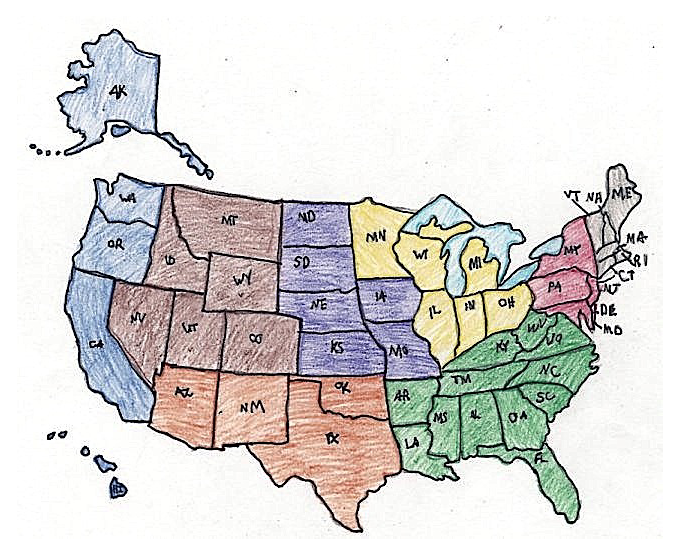
\includegraphics[scale=0.5]{figs/map.eps}
    \label{fig:map}
    \caption{\textbf{Region Map used for State feature binarization}}
\end{figure}

Finally, all dates were consolidated in date ranges. For better perfmance with the logistic regression classifier, which 
is sensitive to variance in feature scale, all values were transformed so that each feature had a mean value of 0 and a 
standard deviation of 1 across the training samples. At this point, any feature that had the same value on every sample 
was discarded.

\subsection{Training}
\label{methods.training}

Once data was processed, the models were ready to be trained. Each of the models has features that must be tuned for optimal 
performance. To mitigate overfitting on the training data, 5-fold cross-validation was used while training each model, using 
the split detailed above. To tune each parameter, a \emph{grid search} was performed for each parameter as follows.

\subsubsection{Logistic Regression}
\label{methods.training.lr}
The logistic regression model had two parameters to tune: the penalty function and the regularization constant \emph(C). The grid 
search was performed with L1 and L2 norms for the penalty function and values of C logarithmically spaced from 0.001 to 1000. The 
best parameters found were an L1 norm with C value of 1 (which were interestingly the scikit-learn defaults). This 
classifier achieved an average accuracy of about 66\% on the training data.

\subsubsection{Random Forest}
\label{methods.training.rf}
Training the random forest classifier involved tuning the number of estimators used, as well as the maximum number of features 
for each estimator to consider. The number of estimators ranged from 10 to 100, while the maximum features were either the 
total number of features, or the square root or base-2 log of this value. The best combination found had 50 estimators with 
a base-2 log of the total features considered by each. This combination achieved an average score of about 82\% training accuracy.


\subsubsection{Gradient Boosting}
\label{methods.training.gb}
Lastly, training the gradient boosting classifier required the tuning of the number of estimators, as well as 
the maximum depth of each. The number of estimators ranged from 100 to 1000, while the maximum depth ranged from 1 to 5. 
The winning combination was 300 estimators with a depth of 2. This also had an average accuracy of around 82\%
on the training data.
